

\begin{frame}{}
    \begin{center}
        \large \textbf{ERNIE 1.0: Enhanced Representations through Knowledge Integration}
    \end{center}
    \vspace{20pt}
    
    \textbf{Author(s):}
    \begin{itemizeSpaced}{5pt}
    {\color{DimGrey} 
    
        \item Sun et al. (2019) in \emph{ERNIE: Enhanced Representations Through Knowledge Integration}
        
    }
    \end{itemizeSpaced}
\end{frame}

% -------------------------------------------------




\begin{frame}{ERNIE: Motivations}

    \vspace{10pt}
    
    \begin{itemizeSpaced}{2pt}
        \pinkbox Previous models (Word2Vec, GloVe, BERT) make embeddings via context and co-occurrence $\Rightarrow$ fail to use prior knowledge (tucked away in sentence ordering and proximity) to capture relationships between entities. 
    \end{itemizeSpaced}

    
    \vspace{-5pt}
    \begin{exampleBlock}{Example: ERNIE's Entity Capturing Skills}
        
        Consider the following training sentence: \newline 
        
        {\footnotesize \textit{``Harry Potter is a series of fantasy novels written by J. K. Rowling."}}\newline 
        
        Using co-occurring words ``J.", ``K.", and ``Rowling", BERT is limited to predicting the token ``K." but utterly fails at recognizing the whole entity \emph{J. K. Rowling}. \newline 
        
        A model could use simple co-occurrence counts to predict the missing entity \emph{Harry Potter} even without using long contexts ... but it would not be using the \emph{\alert{relationship between the novel name and its writer}}. 
    \end{exampleBlock}


    \vspace{-5pt}
    \begin{itemizeSpaced}{2pt} 
        
        \pinkbox {\color{ForestGreen} \textbf{ERNIE to the rescue! }} ERNIE can extrapolate the relationship between the \emph{Harry Potter} entity and \emph{J. K. Rowling} entity using implicit knowledge of words and entities $\Rightarrow$ can predict Harry Potter is a series written by J. K. Rowling (Sun et al., 2019a). 
    
    \end{itemizeSpaced}
    
\end{frame}


\begin{frame}{ERNIE: Phrase and Entity-Level Masking}

    \vspace{10pt}
    
    \begin{itemizeSpaced}{5pt}
        \item ERNIE uses a Transformer Encoder coupled with \textbf{entity-level masking} and \textbf{phrase-level masking} (to encode prior knowledge in {\color{DodgerBlue} conceptual units} like phrases and entities) $\Rightarrow$ learns longer semantic dependencies, has better generalization, adaptability. 
        
        \item \textbf{Phrase-level masking: } A phrase is a ``small group of words or characters acting as a {\color{DodgerBlue} conceptual unit}" (Sun et al., 2019a). ERNIE chunks sentences to find phrase boundaries, then masks and predicts them. 
        
        \item \textbf{Entity-level masking: } name entities contain ``persons, locations, organizations, products." Often include conceptual information. ERNIE parses the entities from a sentence, masks them, then predicts all slots within entities, as shown in \cref{fig:ernie_maskingTypes}.
        
    \end{itemizeSpaced}
    
    
    
    \begin{figure}[h]
    \vspace{-5pt}
    \centering
    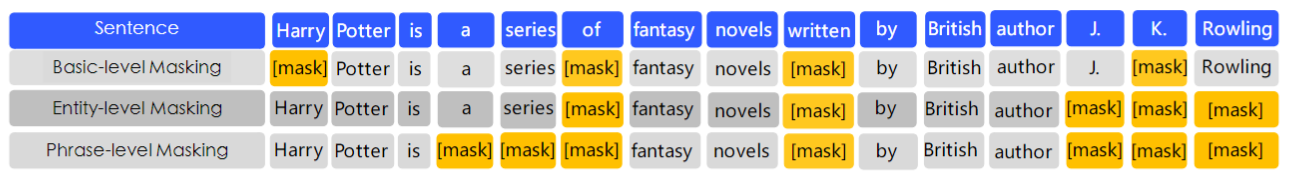
\includegraphics[width=0.99\textwidth]{imgs/ernie_maskingtypes.png}
    \vspace{-5pt}
    \captionof{figure}{\linespread{0.3}\scriptsize ERNIE uses basic masking to get word representations, followed by phrase-level and entity-level masking. From \emph{ERNIE: Enhanced Representation Through Knowledge Integration}, by Sun et al., 2019. \url{https://arxiv.org/pdf/1904.09223.pdf}. Copyright 2019 by Sun et al.}
    \vspace{-5pt}
    \label{fig:ernie_maskingTypes}
    \end{figure}
    
    
\end{frame}



\begin{frame}{ERNIE: Knowledge Learning To Fill-In-Blanks on Named Entities}

\vspace{10pt}

\begin{table}[htbp]
    \scriptsize 
    \centering \linespread{0.3}
    \setlength{\tabcolsep}{4pt} % Default value: 6pt
    \renewcommand{\arraystretch}{3} % Default value: 1
    
    \begin{tableFont}
    \begin{tabu} to \textwidth {| X[0.4] | X[6] | X | X | X |}
        
    
        \hline
      
        %\rowcolor{MyLavender} 
        \centering \textbf{Case}
        & \centering \textbf{Text} 
        & \centering \textbf{ERNIE}
        & \centering\textbf{BERT} 
        & \centering \textbf{Answer} \\ 
        
        \hline
        
        
        $1$
        &
        ``In September 2006, $\_\_\_$ married Cecilia Cheung. They had two sons, the older one is Zhenxuan Xie and the younger one is Zhennan Xie." \newline
        & 
        Tingfeng Xie
        & 
        Zhenxuan Xie
        & 
        {\color{Green} \textbf{Tingfeng Xie}} \\ 
        
        \hline 
        
        
        
        $4$
        &
        ``Australia is a highly developed capitalist country with $\_\_\_$ as its capital. As the most developed country in the Southern Hemisphere, the $12$th largest economy in the world and the fourth largest exporter of agricultural products in the world, it is also the world's largest exporter of various minerals."   \newline 
        & 
        Melbourne
        & 
        (Not a city name)
        & 
        {\color{Green} \textbf{Canberra}} \\ 
        
        \hline 
        
        $6$
        &
        ``Relativity is a theory about space-time and gravity, which was founded by $\_\_\_$."   
        & 
        Einstein
        & 
        (Not a word in Chinese)
        & 
        {\color{Green} \textbf{Einstein}} \\ 
        
        
        \hline 
    \end{tabu}
    
    \end{tableFont}
    
    \vspace{-5pt}
    
    \captionof{table}{\linespread{0.2}\scriptsize Comparing ERNIE to BERT on Cloze Chinese Task. From \emph{Figure 4 in ERNIE: Enhanced Representation Through Knowledge Integration}, by Sun et al., 2019. Copyright 2019 by Sun et al.}
    
    \label{tbl:ernie_vs_bert_knowledgeLearningTask}
\end{table}
\vspace{-10pt}



\vspace{-10pt}
\begin{itemizeSpaced}{0pt}
    \linespread{0.1}
    \item Case 1: ERNIE predicts the correct father name entity based on prior knowledge in the article while BERT simply memorizes one of the sons' name, completely ignoring any relationship between mother and son. 
    
    \item Case 4, 6: BERT fills the slots with characters related to the sentences but not with the semantic concept. 
    
    \item Case 4: ERNIE predicts the wrong city name, though it still understands the semantic type.
\end{itemizeSpaced}

ERNIE's contextual knowledge understanding is far superior to BERT's!
    
\end{frame}